\chapter{Results and Discussion} \label{chap_results}

This chapter will present the results from performance testing our purposed architecture. Section \ref{sec_hardware_resources} will give an analysis of the hardware resource consumption of our accelerator. In Section \ref{sec_result_performance} we will describe the set up for our performance measurements, give an analysis of the performance of our system, and how the accelerator affect the different layer. We will also compare the performance of the system with a software implementation running on a laptop CPU. 

Remember from Section \ref{sec_what_to_accelerate} that we defined layer 1 as C1/S2, layer 2 as C3/S3, layer 3 as C5, and layer 4 as F6.


\section{Hardware Resources} \label{sec_hardware_resources}

As mentioned in Section \ref{sec_zedboard} we used a Zedboard, with an Artix-7 FPGa, for prototyping our suggested architecture. A short overview of the most vital resources available on the Artix-7 can be seen in Table \ref{tab_available_resources}. Table \ref{tab_resource_usage} shows the resource consumption of each accelerator as the number of accelerators increases. The "DSPs: Convoluter" column shows how many DSPs the covoluter module within the accelerator consumes.

As we can see from Table \ref{tab_resource_usage} the convoluter makes heavy usage of the DSPs. In its current state it contains $ 5 \times 5 $ MAC units, which optimally consumes four DSPs each. When the number of available DSPs is reduced, the MAC units need to exchange the DSP with LUTs, which causes an massive spike in resource consumption.

Since the accelerators optimal number of DSPs is 116 out the of 220 available, increasing the number of accelerators from one to two does not cause any critical spike in resource consumption. But the converting of 12 DSPs to LUT logic is still significant, causing a total of 4000 more LUTs being used. It reaches critical levels when we increase the number of accelerators to three, leaving only 50 DSPs to be used by each convoluter. This causes each accelerator to consume 18699 LUTs, giving a total of 56097, which exceeds the maximum of available LUTs by 2897. Thereby limiting the number of accelerators to two, unless we change to a bigger FPGA. While a bigger FPGA, e.g. an Virtex 7, would provide us with more hardware resources, it would also increase the size of the chip and power consumption. Making it unsuitable for mobile applications.

This unexpected consumption of resources is unfortunate, since we would preferably wish to run at least four accelerators in parallel, in order to exploit the bandwidth from all four high-performance AXI4 ports. We have been unable to explore ways to reduce the convoluters consumption of DSPs due to time constraints, but it is definitely something that should be done in future work. 

\begin{table}
	\centering
    \begin{tabular}{| >{\centering\arraybackslash}m{0.7in} |  >{\centering\arraybackslash}m{0.7in} |  >{\centering\arraybackslash}m{0.7in} |  >{\centering\arraybackslash}m{0.7in} |  >{\centering\arraybackslash}m{0.7in} |} 
    \hline
    Nof. accelerators & Slice LUTs & Flip-flops & DSPs & DSPs: Convoluter \\ \hline
    1 & 7986 & 3310 & 116 & 100 \\ \hline
    2 & 9941 & 3310 & 110 & 94 \\ \hline
    3 & 18699 & 3310 & 66 & 50 \\ \hline
    4 & 20971 & 3325 & 54 & 50 \\ \hline
        \end{tabular}
    \caption[Resource usage]{Table showing how the resource usage varies for each accelerator as the number of accelerators increases.}
   	\label{tab_resource_usage}
\end{table}


\begin{table}
	\centering
    \begin{tabular}{| >{\centering\arraybackslash}m{1.0in} |  >{\centering\arraybackslash}m{1.0in} |  >{\centering\arraybackslash}m{1.0in} |} 
    \hline
    Slice LUTs & 53,200   \\ \hline
    Flip-flops & 106,400 \\ \hline
    DSPs & 220 \\ \hline
        \end{tabular}
    \caption[Available resources]{Available resources on the Artix-7 FPGA}
   	\label{tab_available_resources}
\end{table}


\section{Performance} \label{sec_result_performance}

\subsection{Setup}

In order to determine the execution speed and power efficiency of our system we have compared it to the ARM Cortex-A9 CPU on the Zedboard and an ASUS X550JK laptop with a Intel Core i7 4710HQ CPU. Both CPUs ran the pure software implementation of the CNN, while our system used a combination of hardware and software, as described in \ref{chap_method}. The clock speed of the accelerator was set to 100 MHz. We ran our own system with four different configurations:

\begin{itemize}
\item 0 layers. No acceleration. The ARM processor computes the whole network.
\item 1 layer. The accelerator computes C1 and S2 (see Section \ref{sec_network_topology}, while the ARM processor computes the rest. 
\item 2 layers. Accelerating C1, S2, C3 and S4.
\item 3 layers. Accelerating C1, S2, C3, S4 and C5.
\item Two accelerators: 2 layers. Running two accelerators in parallel, both accelerating two layers.
\end{itemize}

In order to determine the energy efficiency of the different systems we used the metric \textit{images/J}, i.e. number of images processed per Joule. We also included a metric for measuring execution speed, using images/second. Despite power efficiency being the main focus of this assignment, execution speed can be interesting for several applications and is closely related to power usage. Note that these images are $ 32 \times 32 $, and thus processing one image corresponds to 331104 multiply-and-accumulate operations. Thus, if one wish to convert the metric images/second to operations/second, one simply need to multiply with that number.

The measurements were done by timing the processing of 10 000 images from the MNIST dataset, while measuring the power consumption. 

Total board power was determined by measuring the voltage over pin 1 and 2 on J21 current sense resistor on the Zedboard during execution. We can then use the following equation to calculate the power consumption:

\begin{equation}\label{eq_power_measurement}
 P = (V_{in}-V_{measured}) \times \frac{V_{measured}}{R}
\end{equation}

Where $ V_{in} $ is the input voltage 12V, $ V_{measured} $ is the measured voltage across the pins, which have a resistance of $ R = 10m\Omega $.

With the FPGA programmed and the accelerator activated the board measured to 4.18 W, while the ARM processor alone measured to 3.82 W. The second core was turned off in both cases. We were unable to measure the power consumption of the laptop directly, and therefore used the power estimation provided by ASUS \cite{ASUS2015}. The laptop CPU uses 47 W, and including RAM, motherboard and various peripherals, we estimate a total consumption of 60W. Do note that this estimate is not completely accurate, and could potentially be lower. 


\subsection{Discussion} \label{sec_result_discussion}

\subsubsection{Analysis of the accelerator's performance}

\begin{figure}[h!]
	\centering
	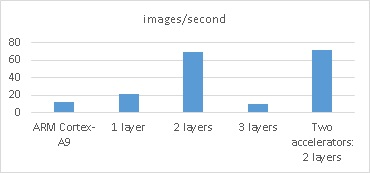
\includegraphics[width=0.8\textwidth]{Figures/Results/results_acc_improvements}
	\caption[Accelerator performance]{Overview of how the performance changes with different configurations of the system, when computing the whole network.}
	\label{fig_results_acc_improvements}
\end{figure}

Figure \ref{fig_results_acc_improvements} shows how accelerating the different layers in hardware affect the performance. We can see that accelerating one layer provides us with a almost 2x speed-up, while accelerating two layers give close to 6x speed-up. In stark contrast, accelerating three layers slows down the system and performs even worse than computing everything in software. We believe this is mainly due to how we move data to the accelerator. Each of the 120 outputs from C5 are computed using the same 16 input maps, but with a different set of 16 distinct kernels. This means that in the current state of our system, we transfer the same 16 input maps 120 times to the accelerator. We consider this a rather ineffective memory access scheme, and purpose a better one in Chapter \ref{chap_future_work}.

Another interesting aspect of Figure \ref{fig_results_acc_improvements} is that running two accelerators in parallel provides virtually no speed-up compared to only running one. There are two feasible explanations for this: 1) the accelerators get starved, i.e. they not fed data fast enough, and 2) the main bottleneck in now layer 3, which reduces the significance of improving performance for layer 1 and layer 2.

In order to determine which layer provided the biggest bottleneck, we decided to measure the performance when removing layer 3 and 4 from the network. I.e. only processing layer 1 and 2. The results can be seen in Figure \ref{fig_performance_C1C2_only_accs}.

Here we see that processing only the first two layers executes 4x faster than processing the whole network. This means that C5/F6 stands for 75\% of the processing time of the whole network. Since C5 has 48120 connections and F6 has 120, it is clear that C5 is the main bottleneck. 

This goes to show that accelerating layer 3 can provide a major boost to the performance of our computing. But, as mentioned, the current scheme we are using to accelerate layer 3 needs to be improved.

In addition, we can see that using the accelerator gives up to 51x speed-up when processing layer 1 and 2. Which demonstrates how much faster the accelerator is than the ARM processor.

\begin{figure}[h!]
	\centering
	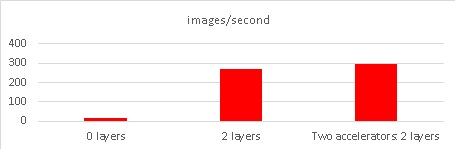
\includegraphics[width=0.75\textwidth]{Figures/Results/performance_C1C2_only_accs}
	\caption[Accelerator performance, layer 1 and 2]{Performance when removing layer 3 and 4 from the network. I.e. only processing layer 1 and 2.}
	\label{fig_performance_C1C2_only_accs}
\end{figure}

But this does not explain why we get so little speed-up when running two accelerators in parallel. Ideally, we should get a 2x speed-up compared to running only one accelerator. In turns out that the DMA bug (see Section \ref{sec_hardware_driver}, which forces us to re-initialize the DMA after it is done processing a BD ring, is part of the explanation. This re-initialization causes the memory needed to store the BD rings for the DMA channels to be reallocated every time, and this takes time. In order to predict the performance if this bug was fixed, we measured the time it took re-initialize the DMA and subtracted it from the execution time. This produced the results seen in Figure \ref{fig_performance_sub_init}.

\begin{figure}[h!]
	\centering
	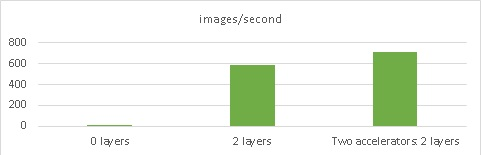
\includegraphics[width=0.8\textwidth]{Figures/Results/performance_sub_dma_init}
	\caption[Accelerator performance, with DMA fix]{Performance when processing only layer 1 and 2, and subtracting DMA initializations.}
	\label{fig_performance_sub_init}
\end{figure}

 We can see that this increases the performance  by more than 2x, and brings the configuration using two accelerators closer to being twice as fast as the one using one accelerator. But we can still see that there is something that is preventing the system to fully exploit having two accelerators running in parallel. We suggest two probable reasons for this:

\begin{enumerate}
\item Currently the processor has to wait for the data transfers to and from the accelerator to finish, without doing anything productively. This causes the accelerators to be starved, since the processors have to set up the transfers while the accelerators do not have to data to consume. Preferably it could set up the other transfers while the accelerator is processing and/or the DMA performs transfers, but due to the initialization bug we have been unable to implement this. 
\item Another fault of the design is that the input buffer to the accelerator has to be filled before it can start processing. A better solution would be to simply stream the data into the accelerator, and make stall when data is not available. 
\end{enumerate}


\begin{figure}[h!]
	\centering
	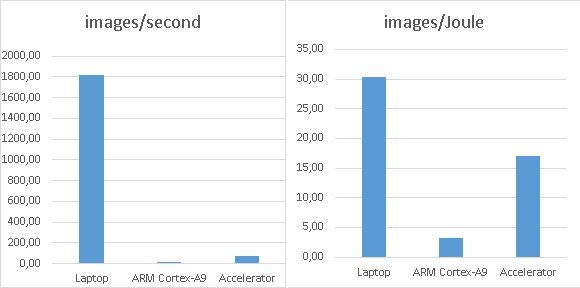
\includegraphics[width=1.0\textwidth,height=5.5cm]{Figures/Results/performance_whole_system}
	\caption[Performance comparison]{Performance when computing the whole network.}
	\label{fig_performance_whole_system}
\end{figure}


\subsubsection{Comparison to a Intel Core i7 4710HQ CPU}

In Figure \ref{fig_performance_whole_system} we can see how our system performs compared to the laptop CPU and the ARM Cortex-A9, when computing the whole network. In this comparison we used our best performing configuration of the system, two accelerators in a parallel that computed layer 1 and 2, while layer 3 and 4 was handled by the ARM processor.

In the current state of the system, it gets handily outperformed by the laptop. The laptop is 25x faster than our system, and almost 2x as power efficient. The reason for this is the bottleneck created by layer 3 and 4, which is computed by the ARM processor.

\begin{figure}[h!]
	\centering
	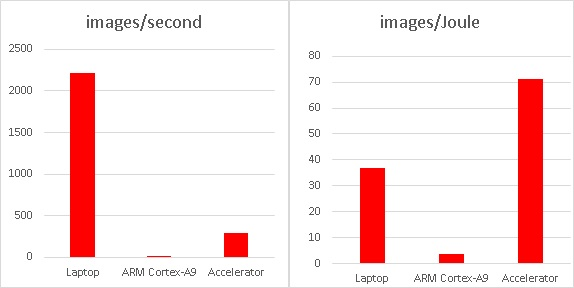
\includegraphics[width=1.0\textwidth,height=5.5cm]{Figures/Results/performance_C1C2_laptop}
	\caption{Performance when only processing layer 1 and 2.}
	\label{fig_performance_C1C2_laptop}
\end{figure}


If we instead of comparing the performance of the whole network, compare the performance when computing layer 1 and 2, our accelerator do much better. As we can see from Figure \ref{fig_performance_C1C2_laptop}, our accelerator is now 7.5x times slower than the laptop, but 2x as power efficient. If we also subtract the performance loss caused by the DMA initialization bug, our accelerator become 5x as power efficient as the laptop. This basically means if our accelerator is going to compete with a state of the art CPU, it has to be extended to it can effectively compute layer 4.  

But despite it not being able to out-perform a laptop CPU, our accelerator would still do better on mobile platforms with power budgets. Our whole system uses 4.18 Watt, while the laptop CPU itself uses 47 Watt. It should also be noted that our system is only a prototype, and there are multiple optimizations that can be done in order to boost performance. Chapter \ref{chap_future_work} will discuss these optimizations.
